\begin{figure}[!h]
\centering
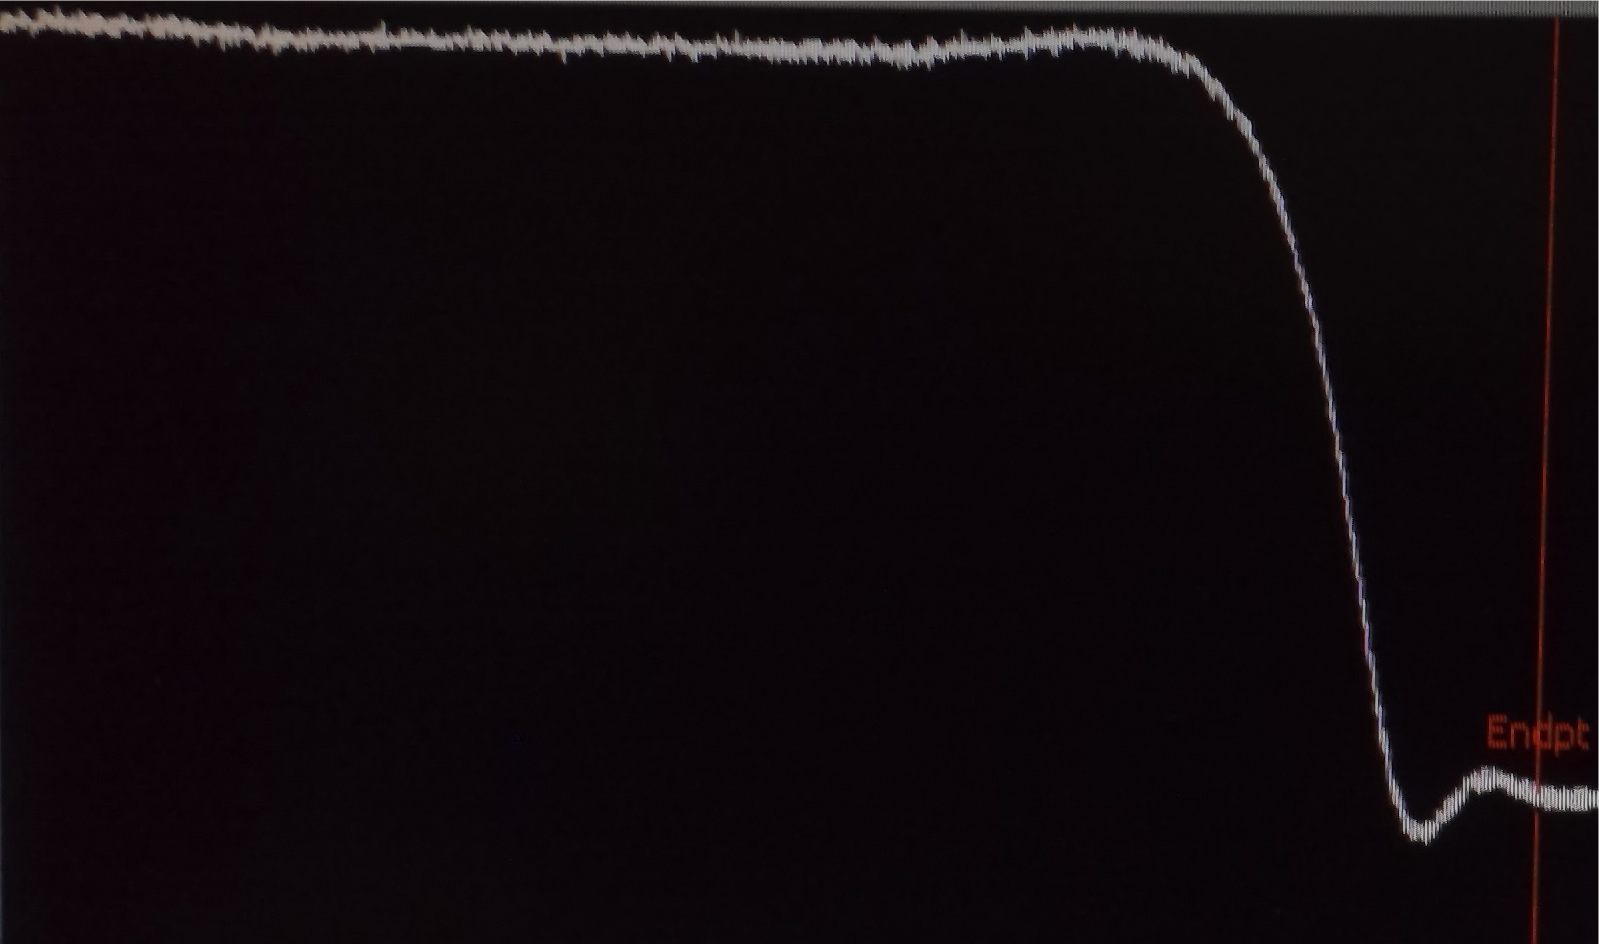
\includegraphics[width=14cm]{figures/plasmatherm_Nb_sloped_endpoint.png}
\caption{\label{fig:plasmatherm_Nb_sloped_endpoint}Typical endpoint signal of Nb etch. The small peak after the dip is interpreted as the end of the etch. Endpoint is called 10\,s-20\,s after that.}
\end{figure}

\begin{itemize}
\item Spin: SPR600 @ 3000\,rpm
\item Expose: 220\,mJ/cm$^2$
\item Develop: double puddle, 30\,s, 30\,s
\item Run through spin rinse dry
\item Inspect with microscope
\item Etch with PlasmaTherm
\begin{itemize}
\item Recipe: 150mm\_Nb\_sloped\_ManEP
\begin{itemize}
\item SF$_6$: 40\,sccm
\item O$_2$: 16\,sccm
\item RF: cut after strikie
\item ICP: 500\,W
\item Pressure: 6.5\,mTorr
\item He: 4\,Torr
\item Rate: $\sim$\,0.51\,nm/s; $\sim$\,31\,nm/min
\item Note: Selectivity over resist is poor; limit to 300\,nm Nb to be etched
\end{itemize}
\item Etch: $\sim$230\,s
\item No DC bias
\item Use endpoint; typical signal shown in Fig.\,\ref{fig:plasmatherm_Nb_sloped_endpoint}
\item Insert picture of endpoint signal and log book entry
\end{itemize}
\item Ash: 2\,min
\item Clean: acetone dirty 2\,min, acetone clean 2\,min, IPA, spin rinse dry
\item Inspect with microscope
\item Measure thickness with profilometer
\end{itemize}



